
Now that we have our model all defined, we can train it. To do this, we will create a \code{Trainer} class that takes in a parameterized model and the path of a directory to save its parameters after each file it trains over. The class will have one method, \code{train}, that takes in a directory of training files, the sample size, and the number of epochs. Because of the complexity of the model, we also want the option to train forever until interrupted. To accomplish this, we will set the default number of epochs to \code{None} and set an infinite loop with a counter and a break.

\begin{minted}{python}
import WaveNet.data as data

class Trainer:
    def __init__(self, model, save_dir):
        self.model = model
        self.save_dir = save_dir

    def train(self, dir, sample_size, epochs=None, verbose=False, timer=False):
        '''
        Trains the model from files in the given directory

        Args:
            dir (str)         : Path to training files
            sample_size (int) : Number of samples in each file section, None for whole file
            epochs (int)      : Number of epochs to train, None to run until stopped
            verbose (bool)    : Should this print extra info about dilating and optimizing?
            timer (bool)      : Should this print extra info about the time taken to calculate?

        Returns: List of losses
        '''
        loader = data.WNLoader(dir, self.model.receptive_field, sample_size=sample_size)

        counter = 1

        while True:
            if epochs is not None and counter > epochs:
                break

            print('='*10, 'Epoch {}'.format(counter), '='*10)
            file_counter, epoch_losses = 1, []

            # Loop through the files
            for file in loader:
                print('\tFile {}'.format(file_counter))

                # Loop through the sections of each file
                for inputs, targets in file:
                    loss = self.model.train(inputs, targets, verbose=verbose, timer=timer)
                    epoch_losses.append(loss)
                file_counter += 1
                self.model.save(self.save_dir, step=file_counter)
            counter += 1

        return epoch_losses
\end{minted}

Now the only thing we need is data. To do this we're going to use torchaudio's datasets, specifically one called CMU Arctic bdl, which is more than a thousand clips of an American man reading short fragments of public domain books. To perform the training, we will write a short script to download the files --- about 98 megabytes worth --- and train over them:

\newpage
\begin{minted}{python}
import WaveNet.WaveNet as WaveNet
import WaveNet.trainer as trainer
import warnings
from torchaudio.datasets import CMUARCTIC

if __name__ == '__main__':
    # The sox backend is deprecated, but we can ignore that for now
    warnings.filterwarnings("ignore")

    # download data
    CMUARCTIC(root='./data/', url='bdl', download=True)

    # Initialize and train the model
    model = Wavenet.WaveNet(5, 12, 256, 512)
    print('Receptive Field:', model.receptive_field)
    trainer = trainer.Trainer(model, './model_saves/')
    trainer.train('./data/ARCTIC/cmu_us_bdl_arctic/wav/', 25000, epochs=1, timer=True)
    
>>> python train.py
Receptive Field: 20475
========== Epoch 1 ==========
	File 1
		Loss: 5.551476	Time: 6.76 seconds
		Loss: 5.470233	Time: 6.69 seconds
		Loss: 5.474391	Time: 6.49 seconds
		Loss: 5.473541	Time: 6.64 seconds
		Loss: 5.437691	Time: 6.93 seconds
		Loss: 5.322380	Time: 5.71 seconds
Saving model into ./model_saves/
	File 2
		Loss: 5.156125	Time: 6.84 seconds
		Loss: 5.210230	Time: 7.09 seconds
		Loss: 5.179309	Time: 6.64 seconds
		Loss: 5.210064	Time: 6.56 seconds
		Loss: 5.052970	Time: 6.53 seconds
		Loss: 5.000860	Time: 7.55 seconds
		Loss: 4.989880	Time: 7.05 seconds
    ...
\end{minted}



Despite being considered fast as compared to other architectures of the past, it's still \textit{state-of-the-art} fast which means it takes us plebeians days to finish a single epoch. This model will train overnight for 317 randomly selected files, or about a third of an epoch, totalling slightly more than 3000 samples. This turns out to be more than enough for the model to stabilize.

\begin{figure}[h]
    \centering
    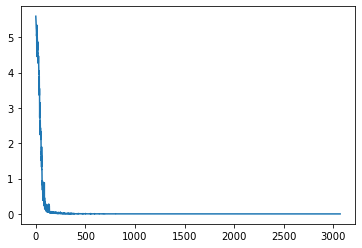
\includegraphics[width=3in]{images/loss.png}
    \caption{Cross Entropy Loss over time}
    \label{fig:loss}
\end{figure}

In Figure \ref{fig:loss}, we can see the loss took a significant drop in the first 500 samples and leveled out after. The limitation of this model is not the amount of data, but computing power. The rate at which this levels off is dependant on the receptive field, itself dependent on the size of the model. It is worth noting that this training could not be done on Google Colab, because the session would crash after eating through all of the available RAM if the receptive field was larger than around ten thousand. Instead, this was done using local runtime.
